\begin{draft}
Este capítulo tem por objetivo detalhar os aspectos do desenvolvimento
do protótipo. Mecânica, o loop de eventos, diagramas entre outros
aspectos do jogo serão abordados aqui.

\section{MECÂNICA}

Para a análise prática das limitações foi escolhido um jogo de
matemática simples. O qual consiste na geração de equações com uma
resposta candidata. Cabe ao usuário informar se o resultado apontado
pelo jogo está correto ou não. A cada resposta dada o nível de
complexidade da equação cresce. O tempo é um fator determinante
no resultado do jogo pois quão mais rápido o jogador acertar se a
afirmação está correta ou não mais pontos ele receberá.

Esta categoria de jogo foi selecionada pois oferece uma experiência
interessante, tem profundidade - oferecendo a possibilidade
de explorar diversos recursos do HTML5. Por ser de razoável
tradutibilidade em tamanhos de telas diferentes e tipos de entrada de
dados diferentes. E, por fim, por oferecer uma dificuldade técnica não
tão desafiadora. Visto que não disponho de experiência profunda no
desenvolvimento de jogos para HTML5.

Jogos como o Math Workout para Android tem uma temática similar.
Não obstante, este jogo não sugere respostas para o usuário
e o questiona sobre a veracidade delas, apresenta apenas a equação
e requer uma resposta. O jogo aqui desenvolvido parece ter uma melhor
jogabilidade para dispositivos móveis, pois não requer a presença
de um teclado. Os botões de verdadeiro ou falso contém todas as
possibilidades.

%Também para não interferir na pesquisa busquei não me distanciar do
%que é considerado padrão em ferramentas e métodos.

%Comecei escrevendo o aplicativo para o Navegador do desktop pois era o
%que estava mais acessível no momento.
\end{draft}

\section{Requisitos}

Abaixo estão dispostos os requisitos do sistema.

\subsection{Requisitos funcionais}

As funcionalidades que o sistema deve apresentar estão descritas abaixo.

\begin{itemize}
    \item O sistema deve prover equações matemáticas de dificuldade crescente para o usuário informar se estão corretas ou não.
    \item O sistema deve pontuar as respostas dadas com maior agilidade com uma pontuação maior, que as respondidas com menor agilidade.
    \item O sistema deve apresentar um ranking com os resultados dos  jogos anteriores.
\end{itemize}

\subsection{Requisitos não funcionais}

Outros aspectos requisitados mas que todavia não fazem parte da regra de negócio.

\begin{itemize}
    \item O sistema deve ser desenvolvido utilizando as ferramentas da web.
    \item O sistema deve funcionar para a plataforma desktop e Android.
    \item O sistema deve ser desenvolvido sem a utilização de nenhuma biblioteca ou framework.
\end{itemize}

\section{Modelagem}

Abaixo segue o diagrama de classes simplificado.

\begin{figure}
    \centering
    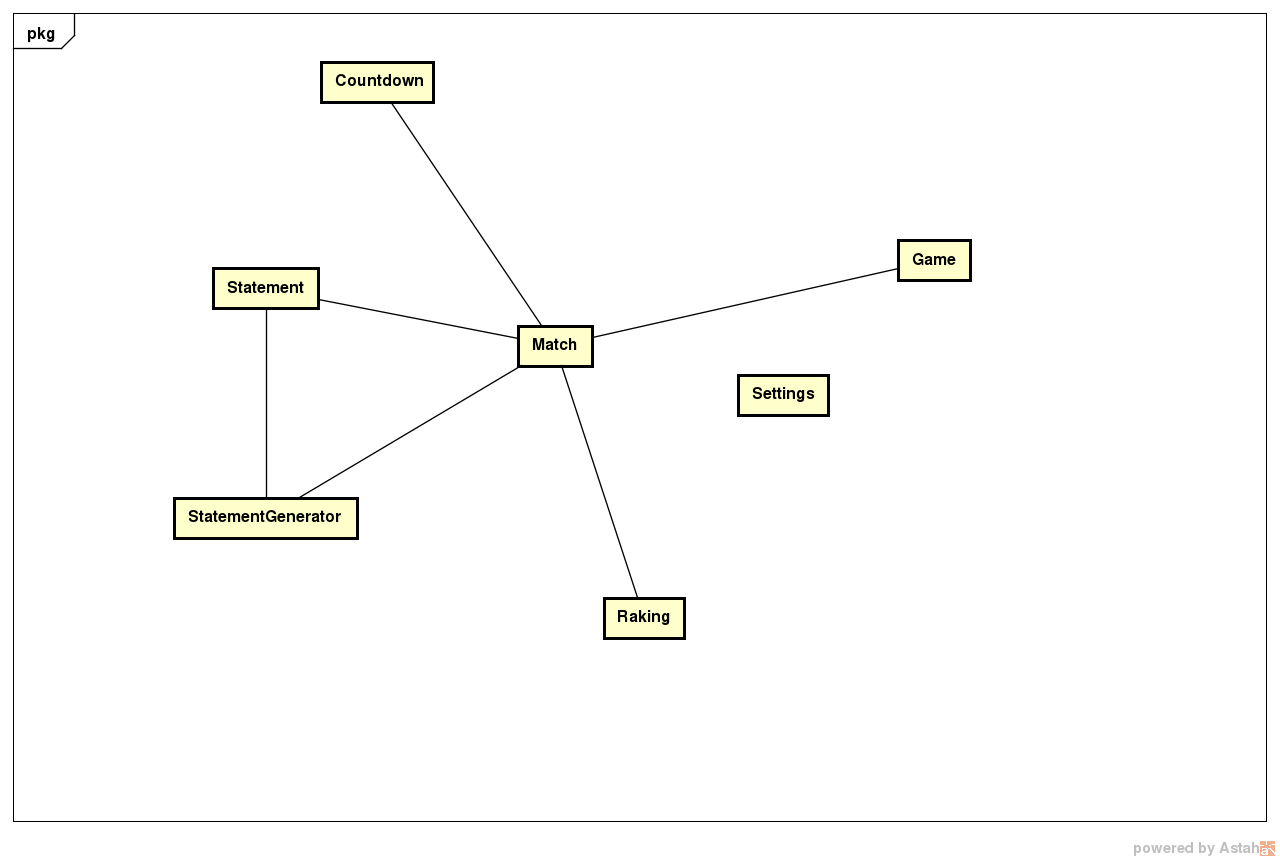
\includegraphics[width=0.8\textwidth,natwidth=610,natheight=642]{ClassesSimpleView.png}
	\caption{Diagrama de classes simplificado}
\end{figure}

Nos anexos pode-se encontrar a versão completa.

\section{Desenvolvimento}

O desenvolvimento se deu com a estratégia de melhoria progressiva.
Desenvolvendo a versão mais simples possível para atingir as
requisitos funcionais. Essa versão mais simples, apesar de não ter
sido testado, deve funcionar na grade maioria dos navegadores.

O primeiro passo foi a criação do documento HTML. Utilizei divs
para simbolizar telas do jogo. Caracterizando o jogo como uma
aplicação SPA (\textit{Single Page Application}).  A alternativa
seria depender de um servidor para mandar as páginas prontas,
mas isso acarreta na necessidade de acesso à internet constante,
coisa nem sempre viável em dispositivos móveis.

Seguindo a construção do markup, veio o desenvolvimento da 
classe Match, a qual simboliza uma partida dentro do jogo.

No início da construção não  havia um gerador de equações, o jogo
contava apenas com um vetor de equações pré-estabelecidas que
eram selecionadas aleatoriamente a cada turno.

Isso se provou uma boa escolha pois possibilitou que o desenvolvimento
se focasse em outros aspectos importantes como a elaboração do laço do jogo.

\section{Laço do jogo}

O laço do jogo (\textit{game loop}) é peça central em praticamente
qualquer jogo eletrônico. A cada iteração do jogo o laço é
executado e o processamento de entrada de usuário e computações
correlacionadas são executadas.

Para escrever o laço é possível utilizar as funções do JavaScript
\textit{window.settimeout}. Não obstante, a forma mais recomendada é
utilizar o \textit{window.requestAnimationFrame} reduz ou completamente
para a execução do laço enquanto o usuário está em outra aba.
Isso reduz o consumo de bateria, uma característica importante para
dispositivos móveis.

O aspecto central do laço do jogo consiste em apresentar uma equação
ao usuário com a possibilidade de ele responder se ela está correta ou
errada.

Uma estratégia interessante que foi adotada na construção foi
declarar todos os objetos relativos ao objeto window. Isso se demonstrou
uma boa forma de separar os objetos, tornando o conflito de variáveis
globais um problema irrelevante.

Outro aspecto positivo foi a utilização de um meta objeto para encapsular
os demais, neste caso utilizei o nome MyMath, funcionando como um namespace,
garantindo que problemas de conflitos de nomes não aconteçam.

Devido ao fato deste trabalho explorar as limitações dos jogos em
HTML5, optei por evitar a utilização de plugins e ferramentas de
terceiros que pudessem ocultar alguma limitação.

Escolhi a simplicidade para não precisar ficar muito tempo aprendendo
as coisas em detrimento do refinamento da pesquisa.

Como armazenamento local foi optado por Web Storage por ser uma API simples,
visto que os requerimentos do protótipo não demandam grande performance ou
armazenamento massivo de dados a opção mais modesta foi preferida.

\begin{figure}
    \centering
    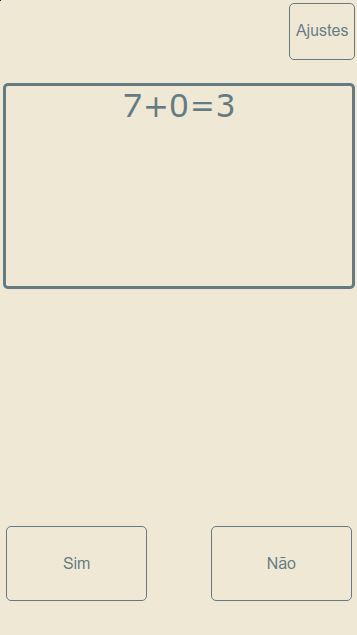
\includegraphics[width=0.8\textwidth,natwidth=610,natheight=642]{board.png}
	\caption{Tabuleiro do jogo}
\end{figure}

\begin{figure}
    \centering
    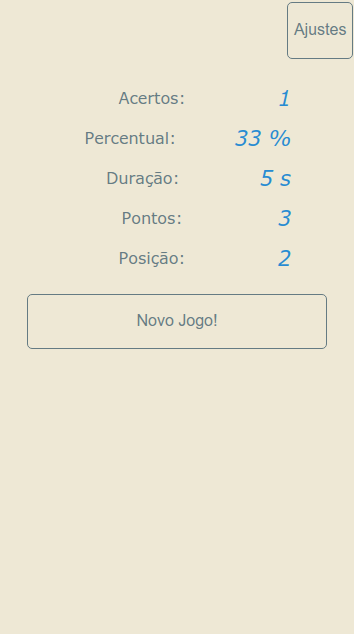
\includegraphics[width=0.8\textwidth,natwidth=610,natheight=642]{score.png}
	\caption{Placar do jogo}
\end{figure}

\begin{figure}
    \centering
    
\includegraphics[width=0.8\textwidth,natwidth=610,natheight=642]{settings.png}
	\caption{Configurações do jogo}
\end{figure}


\section{Otimizações para jogos}


Navegadores tentam otimizar a experiência de navegação definindo
um conjunto de regras e configurações razoáveis para a maioria dos
casos. Não obstante, nem sempre estes valores padrões são as melhores
opções no contexto de jogos. Abaixo segue uma lista de configurações
interessantes para se fazer com CSS no contexto de desenvolvimento de
jogos.
Abaixo seguem algumas otimizações que foram utilizadas no jogo, e são  aplicáveis 
em grande parte dos jogos.


\subsection{CSS}

Scroll é um recurso interessante para longas páginas de texto,
o mesmo não se pode dizer à respeito de jogos.
Principalmente aqueles dependente de contato com a tela, pois
no contato a tela pode se mover e desconcentrar o usuário. Para
remover este comportamento deve-se utilizar o \textit{overflow:
hidden;} do seletor do corpo do documento (\textit{body}).

A barra de endereço é outro recurso de pouca utilidade no contexto de
jogos, e muitas vezes um empecilho para jogos em dispositivos móveis,
devido ao limitado tamanho da tela.

Para desabilitar a barra em dispositivos da Apple pode-se utilizar a
seguinte configuração:

\begin{verbatim}
<meta name="apple-mobile-web-app-capable" content="yes" />
\end{verbatim}

Para os demais dispositivos não existe meio oficial de esconder a barra
de endereço. Não obstante, alguns sites recomendam a solução descrita abaixo:

\begin{verbatim}
<body onload="setTimeout(function() {window.scrollTo(0, 1)}, 100)">
</body>
\end{verbatim}

Apesar de não fazer parte da especificação, a maioria dos navegadores
implementa a possibilidade de desativar a seleção de elementos na tela.
Em jogos essa possibilidade é útil, pois não é natural a seleção de texto
neste tipo de software. \cite{html5mostwanted} cita que desabilitar
a seleção de texto em jogos é uma otimização importante para a
experiência do usuário. Para desabilitar pode-se utilizar as regras
CSS demonstradas abaixo.

\begin{verbatim}
-moz-user-select: none;
-webkit-user-select: none;
-ms-user-select: none;
\end{verbatim}

\subsection{JavaScript}

\subsubsection{Modo estrito}
Algumas das recomendações nesta seção podem não se aplicar
exclusivamente ao desenvolvimento de jogos. Outrossim são de grande
relevância para a criação de sistemas de grande complexidade em geral,
característica comum da grande maioria dos jogos.

Um recurso interessante do JavaScript é seu modo estrito, este faz
um conjunto de modificação na semântica do interpretador de modo
que alguns recursos suportados, mas propensos a problemas, sejam
desabilitados. Um exemplo é variáveis sem o prefixo var.

O modo estrito pode ser entendido como uma variante mais rígida
do JavaScript. O modo restrito pode ser habilitado utilizando o
termo \textit{"use strict";} nos cabeçahos de arquivos ou funções
permitindo que código não estrito trabalhe em conjunto com código
estrito, característica conveniente para a utilização em sistemas
legados.

\subsubsection{Funções imediatamente invocadas}

Um problema comum de sistemas complexos em JavaScript é que muitos
objetos vivem em ambiente global. Isso pode causar uma coleção de
problemas, desde conflitos de nomes à sobrescrita de variáveis. Para
contornar esse problema pode-se utilizar as funções imediatamente
invocadas IFE (\textit{Immediatly invoked function expression}).

\begin{figure}
\centering
\begin{verbatim}
    (function() {
        'use strict';

        function bar() {
            return 'foo';
        }

        window.bar = bar;
    })();
    window.bar();
\end{verbatim}
\caption{Exemplo de utilização de funções imediatamente invocadas}
\label{fig:iife}
\end{figure}

A figura \ref{fig:iife} demonstra a utilização deste padrão. As
funções definidas no mesmo nível que bar não estarão no contexto
global - a não ser que seja especificado diretamente - e não sofrerão
conflitos de nomes e outros problemas relativos ao contexto global.

\subsubsection{HTML}

Um problema que jogos sofrem em geral é a demora no carregamento da
grande quantidade de recursos que precisam estar em memória para o jogo
funcionar. Muitos jogos utilizam uma tela de carregamento enquanto os 
recursos são adquiridos. 

Um recurso do HTML interessante para este tipo de situação é o pré carregamento
de recursos (\textit{Link Prefetching}). Esta tecnologia possibilita que o navegador
, em seu tempo livre, adquira recursos que provavelmente serão necessários em um futuro próximo.

Nem todos os recursos necessitam ser pré carregados, mas uma impressão
muito superiora é criada se os recursos estão imediatamente
disponíveis quando uma nova fase é carregada \autocite[pp. 39]{creatingFun}.

